\chapter{Programming project description}
\label{chap:project}
\section{Introduction}

Programming project of this thesis is a set of command line programs, collectively
called \emph{Karstgen}, that take
the description of karst cave fracture net and generate polygon mesh in
simple and popular Wavefront OBJ textual file format\footnote{\url{http://www.martinreddy.net/gfx/3d/OBJ.spec}}.

Models created this way may be opened in 3D editing program for further editing
and examination.

Karstgen can also create models for \emph{Vorticity} game engine that was created
by the author together with mr Michał Siejak for graphics related courses\footnote{Computer
  Graphics and Visualiation, summer semester 2009/2009 and Group Project, summer
semester 2009/2010} during licenciate studies at Adam Mickiewicz University \todo{check form}of
Poznań.

\section{Architecture}

Karstgen was created with Unix Philosophy in mind \parencite{raymond2003art}.
It is made of two programs named \emph{blobber} and \emph{mcblob} that have
clearly defined reposinsibilities and communicate through simple textual data
format.  Both programs may take input either from files or from standard input
so they can be piped together with shell pipes. Data flow of karstgen is
presented in \autoref{fig:karstgenflow}.
\begin{figure}[ht]
  \begin{center}
    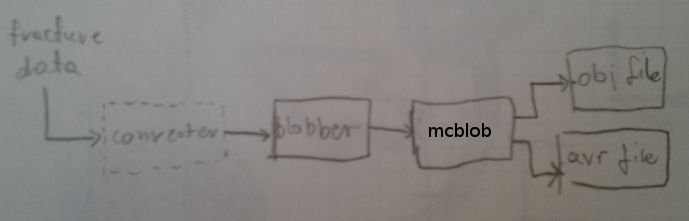
\includegraphics[width=\textwidth]{chapters/project/karstgenflow.jpg}
  \end{center}
  \caption{Data flow of karstgen program. Converted from some other possible
  format is not part of the project.}
  \label{fig:karstgenflow}
\end{figure}
\todo{replace \autoref{fig:karstgenflow} with TikZ graphics}

\subsection{Blobber}
Blobber takes description of a fracture net in a simple textual format and
generates list of metaballs (see \autoref{sub:metaballs}). It can
optionally tilt positions and sizes of metaballs in random but adjustable manner
for more natural--looking results. Blobber also controls quality of the final
geometry. For information about runtime parameters invoke
\begin{verbatim}
./blobber --help
\end{verbatim}

\subsection{Mcblob}
Output generated by blobber is consumed by program named \emph{mcblob}\footnote{Marching
Cubes from blobs} that is in fact a general purpose tool that may be used to
generate geometry from a list of metaballs in 3D space.

\section{Implementation}
\subsection{Metaballs}
Implementation heavily relies on rendering with metaballs. Metaball is a scalar
function in the form:
\begin{equation}
  f(x,y,z)=\frac{d}{(x-x_0)^2+(y-y_0)^2+(z-z_0)^2}
  \label{eq:metaball}
\end{equation}
where $(x_0,y_0,z_0)$ is the center of the metaball and $d$ is a multiplier that
controls the size of the metaball.

If more than one metaball is present in the scene, density function (see Definition
\autoref{def:density function})
is in the form:
\begin{equation}
  d(x,y,z) = \sum_{i=0}^{n} f_i(x,y,z)
  \label{eq:metaballdensity}
\end{equation}
where $n$ is the total number of metaballs in the scene and $f_i$ is function~\ref{eq:metaball}
of the $i$-th metaball.

Metaballs were discovered by Jim Blinn when he was working on visualisation of
molecular structures \parencite{Blinn:1982:GAS:357306.357310}.
\todo{add input file to thesis}
\label{sub:metaballs}
\begin{figure}[htb]
  \begin{center}
    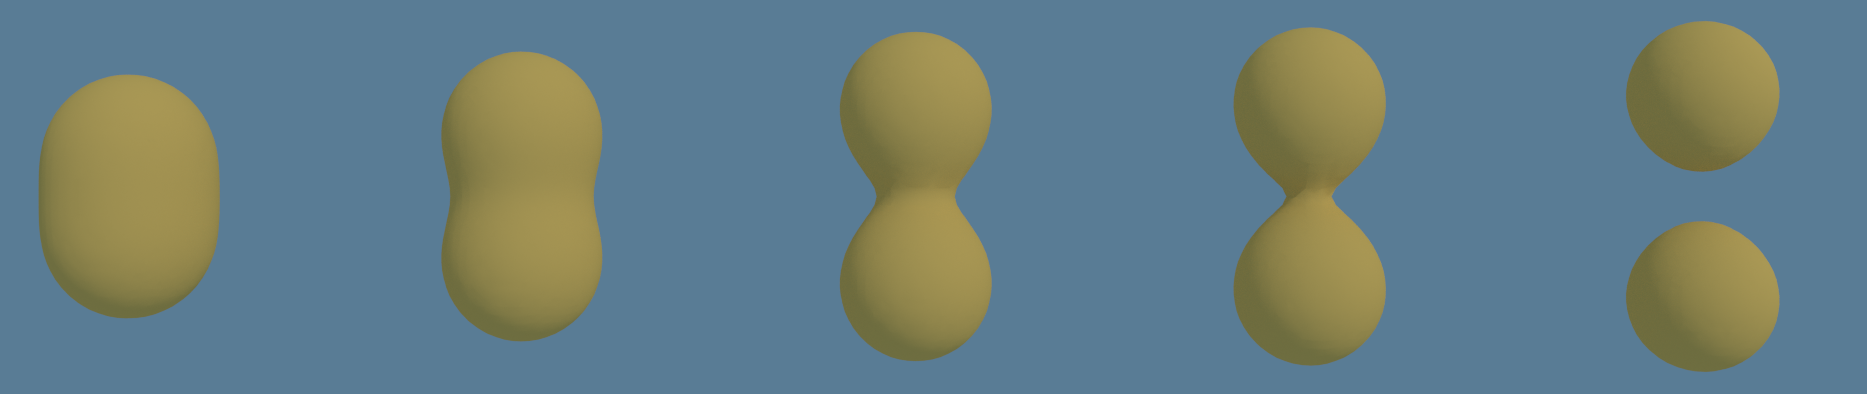
\includegraphics[width=\textwidth]{chapters/project/metaballs.png}
  \end{center}
  \caption{Two metaballs at various distances showing how they are ,,melitng''
    together when getting closer to each other. Geometry was generated with
    \emph{mcblob} program and final image was rendered with Blender 2.68 with
    Cycles renderer. Input file for mcblob that generates this is included with the thesis
      in \texttt{mcblob.in} file.
  }
  \label{fig:metaballs}
\end{figure}

They have the interesting property of ,,melting'' when getting close together
forming structure with somewhat ,,organic'' look and feel (see \autoref{fig:metaballs}).

\subsection{Overview}
Both blobber and mcblob are implemented in C++ language with latest C++11
version of the standard. Build system used to compile the code is \emph{CMake}\footnote{Cross--platform make}
-- meta build syste that can generate native projects for various IDEs and
actual build systems.
Executables use \emph{Boost Program Options} library for parsing command line
arguments and providing help.

Karstgen uses unit testing framework \emph{Google~Test}\footnote{\url{http://code.google.com/p/googletest/}}.
Documentation is automatically generated from sources with Doxygen
tool.


\subsection{Blobber}

For vector data structuers blobber uses \emph{GLM}\footnote{\url{http://glm.g-truc.net/0.9.4/index.html}}
-- a mathematical library that resembles GLSL\footnote{OpenGL Shading Language}.

It reads information about diameters of fractures in fractures network
and places blobs along these fractures with diameters roughly the same as of
these fractures.

Blobber works on structure calleed \texttt{DataPoint}:

\begin{lstlisting}
struct DataPoint
{
  	int x, y, z;
	float midDiam;
	std::vector<float> xData;
	std::vector<float> yData;
	std::vector<float> zData;
};
\end{lstlisting}

This structure can describe three fractures originating in index $(x,y,z)$ in
the fracture net and going along each axe in ascending direction. Each fracture
is described as a vector of uniformly distributed diameters. If there is only
one diameter in a vector it is assumed that the fraction it represens has the
same diameter along its whole length. When no diameters are present in some
vector it is assumed that there is no fracture in this direction.
Additional field \texttt{midDiam} is a diameter of blob that should be placed in
the intersection of the three fractures.

\begin{figure}[hbt]
  \begin{center}
    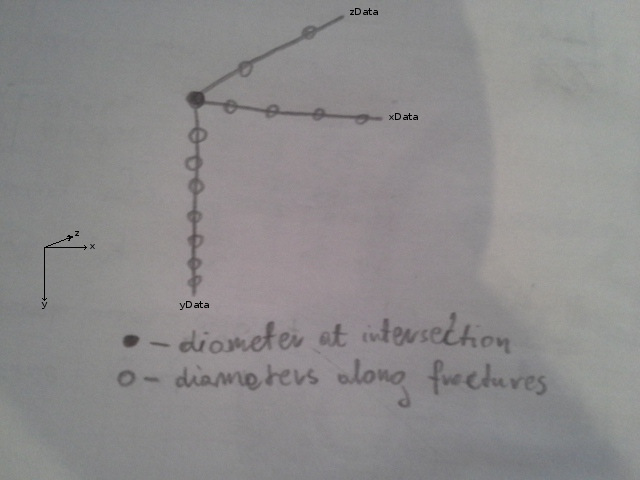
\includegraphics[width=0.7\textwidth]{chapters/project/datapoint.jpg}
  \end{center}
  \caption{Graphical representation of \texttt{dataPoint} -- a basic structure that
blobber works on}
  \label{fig:datapoint}
\end{figure}

Data points are packed into a structure representing whole fracture network
called \texttt{FractureNet}:
\begin{lstlisting}[label={lst:fracturenet},escapeinside={@}{@}]
struct FractureNet
{
	//size of net in number of dataPoints
	int x; int y; int z;
	
	//length of single fracture in each direction
	float xLen; float yLen; float zLen;
	
	std::map<std::tuple<int, int, int>, DataPoint> dataPoints;
};
\end{lstlisting}

Since fracture net is usually quite sparse dictionary structure
(\texttt{std::map} from STL\footnote{Standard Template Library} exactly) is
used to store data points instead of array or vector. Keys in this dictionary
are tuples containing 3D index in a fracture net. This way, given one data point
it is easy to find its neighbours.

\subsubsection{Placement of blobs}

Blobber works on one data point at a time through \texttt{blobsFromDataPoint()}
function. First, one point is placed in the intersection of the axes with
diameter equal to \texttt{mid\-Point\-Diam}. Then, vector for each non--empty
axe is processed by \texttt{blobsOnVector()} function. Besides the vector of
diameters, this function takes \texttt{midPointDiam} of the data point, and optionally
\texttt{nextDpMidDiam} which is \texttt{midPointDiam} of the next data point
along this axis if such data point exists. Fast lookup of next data point is
is possible thanks to dictionary storage. If there is no neighbour data
point at the end of the axis \texttt{nextDpMidDiam} is considered to be 0.\todo{test if this makes sense}

\begin{figure}[htb]
  \begin{center}
    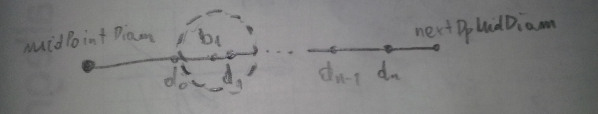
\includegraphics[width=\textwidth]{chapters/project/placement.jpg}
  \end{center}
  \caption{Blobs are placed along fracture defined as set of diameters
    $(d_0,d_1,\cdots,d_{n-1})$. In this example diameter of blob $b_1$ will be a
    linear interpolation of diameters $d_0$ and $d_1$ proportional to distance
    from these diameters.}
  \label{fig:placement}
\end{figure}

Function \texttt{blobsOnVector()} places blobs on the fracture line until
it's wholly covered. Diameters of blobs are determined in a way described
besides \autoref{fig:placement}.

Format of the input to blobber is described in generated documentation:
\begin{verbatim}
\doc\blobber\html\index.html
\end{verbatim}

Output format is the same as input format of mcblob program and is described in
its help:
\begin{verbatim}
./mcblob --help
\end{verbatim}

\subsection{Mcblob}
